\section{Analyse und Planung}
\label{sec:AnalyseUndPlanung}

Nach der Fundierung der Architekturgrundlagen kann mit der Planung der zu
entwickelnden Softwarelösung begonnen werden. Diese Ausarbeitung setzt hierbei
am bereits in der Ausarbeitung "`Unternehmensführung"' entwickelten Konzept und
der daraus resultierenden Problemlösung\footnote{siehe dazu
\citet{unternehmensfuehrung2014}, Kapitel Konzeptionierung} an. Auf dem Konzept
aufbauend wird zunächst eine Analyse der Ist-Situation vorgenommen. Hierbei
können gegebenenfalls Elemente der bestehenden Internetpräsenz der Hochschule
identifiziert werden, welche im Projekt wiederverwendet werden können. In einer
anschließenden Planungsphase werden die Anforderungen an die Anwendung
definiert. Diese Phase wird mit der Erstellung des Lastenheftes und dem
Festlegen der Projektgrenzen abgeschlossen.

\subsection{Ist-Analyse}
\label{sec:IstAnalyse}

Momentan lassen sich Informationen über die angebotenen Studiengänge am Studien-
standort Lingen über die Hochschulseite www.hs-osnabrueck.de abrufen. Die Internetseite bietet dabei zum einen 
weiterführende Links zu den einzelnen Instituten und darüber auch viele Informationen für Unternehmen und Studierende.
Hier werden zum Beispiel Labore, Projekte und Dozenten der einzelnen Institute vorgestellt. Zum anderen werden in einer 
Bildergalerie einzelne Impressionen des neuen Campus dargestellt. Ein Screenshot hiervon ist in \abbildung{Bildergalerie} abgebildet.

\begin{figure}[htb]
\centering
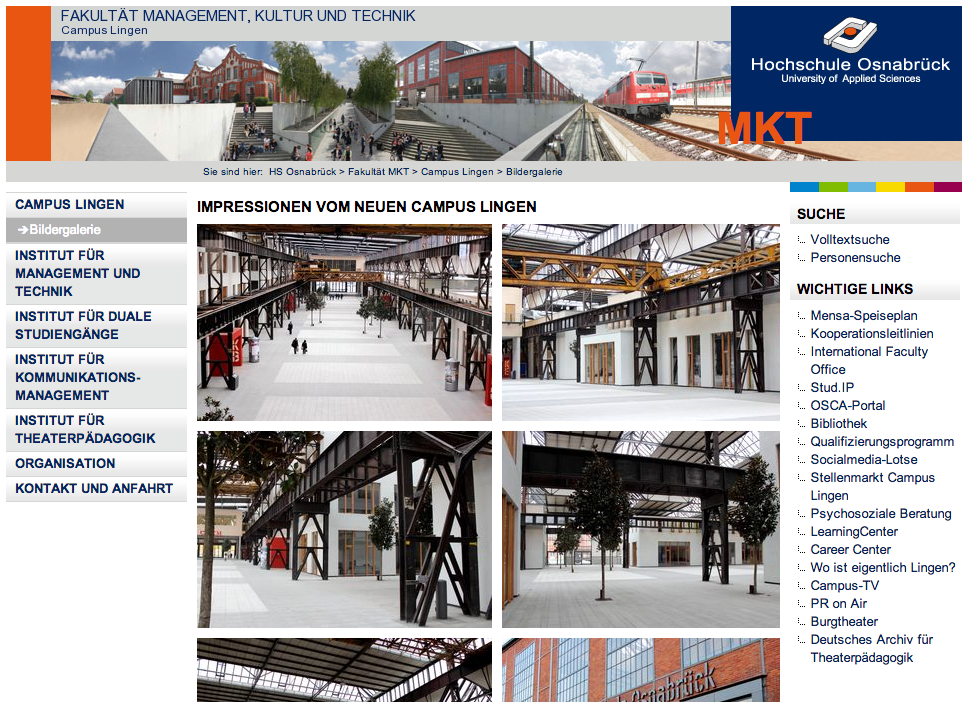
\includegraphics[width=1.0\textwidth]{Bildergalerie.png}
\caption[Bildergalerie des Campus Lingen]{Bildergaliere des Campus Lingen\protect\footnotemark}
\label{fig:Bildergalerie}
\end{figure}
\footnotetext{Link: http://www.campus-lingen.hs-osnabrueck.de}

Ähnlich wie die Informationsvermittlung auf der Internetseite der Hochschule Osnabrück
gestaltet sich auch die Informationsvermittlung auf Messen, auf denen Studieninteressierte
sich auch über die einzelnen Studienstandorte erkundigen können. Dort werden ebenfalls
Impressionen des Campus in Lingen gezeigt oder Informationsmaterial verteilt.

Vor dem Hintergrund der Projektidee, den Campus in 360-Grad Panoramas mit Informationstexten abzubilden, bilden sich aus 
dieser Analyse 2 interessante Elemente heraus.

\textbf{1.} Die Fotos, die bereits vom neuen Campus gemacht wurden.

\textbf{2.} Das Informationsmaterial das über Projekte, Studiengänge, Dozenten und weiteres zusammen getragen wurde.

Die bereits angefertigen Fotos können dabei nicht für das vorliegende Projekt verwendet werden, da es sich bei diesen 
Fotos nicht um 360-Grad Panoramafotos handelt. Darüber hinaus sind auf diesen Fotos nur einzelne Impressionen des Campus 
dargestellt. Das bedeutet die bestehenden Fotos müssten um neu angefertigte ergänzt werden und das ist aus Gründen 
unterschiedlicher Lichtverhältnisse kein sinnvolles Vorgehen. Die bestehenden Impressionen zeigen aber
interessante Blickwickel des Campus. Diese Blickwinkel können bei der Erstellung der neuen Fotos aufgegriffen werden. 

Das zusammengetragene Informationsmaterial kann dagegen aus der Internetquelle der Hochschule verwendet werden, um 
Informationen zu bestimmten Panoramas anzuzeigen. Für die Rechereche nach Informationsmaterial muss daher kein weiter 
Aufwand im Projekt berücksichtigt werden.
\subsection{Lastenheft}
\label{sec:Lastenheft}

% TODO: Verweis auf Unternehmensführung richtig machen
% TODO: Lastenheft hier und im Original überarbeiten!!!!
Nach der Analyse der Ist-Situation gilt es im Folgenden das konkrete Ziel und die Funktionen des Projektes zu definieren. 
Zu diesem Zweck wurde aufbauend auf der Konzeptentwicklung (siehe Kapitel XX Ausarbeitung Unternehmensführung) ein 
Lastenheft angefertigt\footnote{siehe \citet{lastenheft2013}}.

Im Lastenheft ist das folgende Ziel für das vorliegende Projekt definiert:

"`Ziel des Projektes Virtueller Campus Lingen ist es den Standort der Hochschule Osnabrück
in Lingen virtuell darzustellen sowie alle vier Institutionen mit ihren Studienangeboten
vorzustellen."' \footnote{\citet{lastenheft2013}}
Die Darstellung des Campus soll dabei im Stile von Goole Street View\copyright\ in 360-Grad Panoramafotos erfolgen, in 
denen sich ein Nutzer der Software frei umsehen kann. Darüber hinaus soll ein Backendsystem zur Pflege und Wartung der 
Software entwickelt werden\footnote{\citet{lastenheft2013}}.

Zur Erfüllung der Zielbestimmung des Lastenheftes sind darin folgende Produktfunktionen definiert:

\textbf{Benutzerfunktionen}:

\begin{description}
  \item[LF0010] Einem beliebigen Internetnutzer muss es möglich sein, ohne Anmeldung auf die Anwendung zugreifen zu können.
  \item[LF0015] Beim Starten der Anwendung soll dem Benutzer ein 360-Grad Panorama vom Eingangsbereich des Campus Lingen 
  präsentiert werden.
  \item[LF0020] Der Benutzer muss sich in den 360-Grad Fotos der Anwendung frei umsehen können.
  \item[LF0030] Der Benutzer muss zwischen den Fotos navigieren können.
  \item[LF0040] Die Anwendung muss eine Übersichtkarte enthalten, die sowohl den aktuellen Standpunkt, als auch alle 
  weiteren Einstiegspunkte umfasst.
  \item[LF0050] Die Übersichtskarte stellt alle Gebäude des Campus Lingen in Vogelperspektive dar. Innerhalb der 
  Übersichtskarte sind alle Einstiegspunkte in die 360-Grad-Ansicht enthalten.
  \item[LF0060] Die Minimap soll in der oberen linken Ecke des 360-Grad-Fotos angezeigt werden.Sie stellt einen Ausschnitt 
  der Übersichtskarte dar.
  \item[LF0070] In den 360-Grad-Fotos müssen relevante Informationen zu den dargestellten Örtlichkeiten angezeigt werden können.
\end{description}

\textbf{Backendfunktionen}:

\begin{description}
  \item[LF1010] Die Anwendung muss durch den Administrator offline geschaltet werden können.
  \item[LF1020] Der Administrator muss neue Fotos in die Anwendung einpflegen können. Die Fotos können hierbei an beliebigen Punkten auf einem Wegenetz positioniert werden.
  \item[LF1025] Ein Wegenetz muss dem Administrator als Positionierungseinschränkung für neue 306-Grad-Fotos zur Verfügung stehen.
  \item[LF1030] Der Administrator muss veraltete Fotos in der Anwendung austauschen können.
  \item[LF1040] Der Administrator muss Informationstexte zu den 360-Grad-Fotos hinzufügen, abändern und löschen können. Diese Informationstexte können zum Beispiel Projektvorstellungen enthalten. Der Informationstext besteht aus einem Pop-Up mit Einführungstext und weiterführenden Links.
  \item[LF1110] Der Administrator muss sich mit einem Passwort authentifizieren können.
  \item[LF1120] Der Administrator muss das Passwort abändern können.
\end{description}

Diese Funktionen sind zur Erfüllung der Zielsetzung zu implementieren. Neben diesen Funktionen gehen aus dem Lastenheft 
auch folgende Produktdaten hervor:

\begin{description}
  \item[LD0010] 360-Grad Fotos
  \item[LD0020] Informationstexte zu den 360-Grad-Fotos
  \item[LD0030] Benutzername des Administrators
  \item[LD0040] Passwort des Administrators
  \item[LD0050] Wegenetz
\end{description}

Diese sind vor dem Hintergrund der späteren Datenbankplanung zu berücksichtigen.
\subsection{Projektgrenzen}
\label{sec:Projektgrenzen}

Nach der Definition der Anforderung im Lastenheft werden an dieser Stelle die
Grenzen des Projektes aufgezeigt, um einen klar definierten Rahmen zu schaffen.

Es ist hierbei nicht Ziel des Projektes den Campus komplett fotorealisitisch
darzustellen. Die Fotos sollen Einblick in jeden Bereich des Campus bieten und
diesen umfassend darstellen. Es soll jedoch soll nicht jeder einzelne Raum in
der Anwendung abgebildet werden. Weiterhin ist es nicht Anspruch an das
Projekt, alle Projekte und Informationen zum Campuslebens in der Anwendung
darzustellen. Das Projekt ist darauf ausgelegt, Nachhaltigkeit in allen
Bereichen der Informationspflege zu bieten. Es ist daher nicht Aufgabe der
Projektgruppe alle Informationsmaterialien zu sammeln und zu pflegen.

